%! TEX program = lualatex

%https://docs.google.com/presentation/d/1KeKwltg6pmg5WHuUKLPaiNXfClF9qF8kOu08yVI0CpI/edit?usp=sharing

\documentclass[nobackground,dvipsnames,table]{beamer}
%\usepackage{sio}
\usepackage{tsc}
\usepackage{pdfpc}
\usepackage{pgfpages}
\usepackage{multimedia}
\captionsetup[figure]{font=footnotesize}

%%%%%%%% edit hyperlink colors %%%%%%%%
\hypersetup{
  colorlinks   = true, 
  urlcolor     = tscurl, % color of external hyperlinks
  linkcolor    = white,   % color of internal links
}

\mode<presentation>
{\usetheme{default}
	\usecolortheme{tsc}
	\setbeamercovered{transparent}
	\useinnertheme[shadow=false]{rounded}
	\usebackgroundtemplate{}
	\setbeamercolor*{frametitle}{parent=palette primary}
	\setbeamerfont{block title}{size={}}
	\setbeamertemplate{navigation symbols}{}
    \setbeamertemplate{itemize items}[circle]
        \setbeamertemplate{enumerate items}[circle]
}
%{\usetheme{Hannover}
%	\usecolortheme{sio}
%	\setbeamercovered{transparent}
%	\useinnertheme[shadow=false]{rounded}
%	\usebackgroundtemplate{}
%	\setbeamercolor*{frametitle}{parent=palette primary}
%	\setbeamerfont{block title}{size={}}
%	\setbeamertemplate{navigation symbols}{}
%}

%%% below command addresses log output error when trying to use \\ in \author %%%
\pdfstringdefDisableCommands{%
  \def\\{}%
}

%%%%%%%%%%%%%%%%%%%%%%%%%%%%%%%%%%%%%%%%%%%%%%%%
%%%%%%%%%%%%%%%%  SLIDE 1  %%%%%%%%%%%%%%%%%%%%%
%%%%%%%%%%%%%%%%%%%%%%%%%%%%%%%%%%%%%%%%%%%%%%%%
\title[Metrics \& Measurement]{Metrics \& Measurement}
%\subtitle{A document made with thought and care}

\author[Goldberger and Leavitt]{Inbal Goldberger (ActiveFence) \\ Alex Leavitt (Roblox / UC Berkeley)}
%\institute[SIO]{\large Stanford Internet Observatory}
\date[]{}
\subject{Trust and Safety}
\AddToShipoutPictureBG*{
  \AtPageLowerLeft{\hspace{-0.4cm}
    
\includegraphics[width=13.1cm]{img/consortium-image}}
}

% Change this to make a file with just slides, just notes or both
%\setbeameroption{hide notes}                 % Only slides
%\setbeameroption{show only notes}            % Only notes
\setbeameroption{show notes on second screen} % Both

\begin{document}

%\coverpage

\begin{frame}
	\titlepage
\end{frame}

%%%%%%%%%%%%%%%%%%%%%%%%%%%%%%%%%%%%%%%%%%%%%%%%
%%%%%%%%%%%%%%%%  SLIDE 2  %%%%%%%%%%%%%%%%%%%%%
%%%%%%%%%%%%%%%%%%%%%%%%%%%%%%%%%%%%%%%%%%%%%%%%
\begin{frame}{Learning objectives}
Today we will:
\begin{itemize}
    \item Learn about metrics, what they are and why they are important
    \item Learn how to measure success in Trust \& Safety and what metrics are used
    \item Discuss metrics and transparency reports
\end{itemize}
\end{frame}

%%%%%%%%%%%%%%%%%%%%%%%%%%%%%%%%%%%%%%%%%%%%%%%%
%%%%%%%%%%%%%%%%  SLIDE 3  %%%%%%%%%%%%%%%%%%%%%
%%%%%%%%%%%%%%%%%%%%%%%%%%%%%%%%%%%%%%%%%%%%%%%%
\begin{frame}{What is a metric?}

\begin{itemize}
    \item “A measurement system that quantifies static or dynamic characteristics”
    \item In practice, metrics…

    \begin{itemize}
        \item Have a definition that can be counted and tracked over time
        \item Are utilized for tracking “success” of goals for a product, policy, etc. over time
        \item Importantly: are useful \emph{when they can be changed}

        \begin{itemize}
            \item ie., a metric should be able to increase or decrease, as a result of either 1) organic human behavior {[e.g., number of users who click on a button]}, or 2) a systems change {[e.g., more people clicked on the blue button than the red button]}
        \end{itemize}
    \end{itemize}
    
    \item {[READING \#1 - Integrity Institute Metrics/Measurement]}
\end{itemize}

\end{frame}


%%%%%%%%%%%%%%%%%%%%%%%%%%%%%%%%%%%%%%%%%%%%%%%%
%%%%%%%%%%%%%%%%  SLIDE 4  %%%%%%%%%%%%%%%%%%%%%
%%%%%%%%%%%%%%%%%%%%%%%%%%%%%%%%%%%%%%%%%%%%%%%%
\begin{frame}{Examples of Generic Platform Metrics}

\begin{itemize}
    \item Growth

    \begin{itemize}
        \item “DAU” - Daily Active Users

        \begin{itemize}
            \item Keeps track of the number of people who have active accounts on a platform

        \end{itemize}
        
        \item Clickthroughs

        \begin{itemize}
            \item Keeps tracks of how many times people interact with a link, button, etc.
        \end{itemize}
    \end{itemize}
\end{itemize}

\end{frame}


%%%%%%%%%%%%%%%%%%%%%%%%%%%%%%%%%%%%%%%%%%%%%%%%
%%%%%%%%%%%%%%%%  SLIDE 5  %%%%%%%%%%%%%%%%%%%%%
%%%%%%%%%%%%%%%%%%%%%%%%%%%%%%%%%%%%%%%%%%%%%%%%
\begin{frame}{Why measure metrics for Trust \& Safety?}
\begin{itemize}
    \item Taking a step back: making the case for T\&S - why is T\&S important?

    \begin{itemize}
        \item Our ultimate target in T\&S: user trust, civil communication, healthy interactions, sense of safety 
        \item Conceptually we understand the link between high user trust and higher engagement, more advertisement and overall community prosperity
    \end{itemize}

    \item Historical view - T\&S perceived as a “cost center”. i.e. It takes money from the company through disabling Ads, blocking accounts, reducing engagement.

    \begin{itemize}
        \item There was a need to show how T\&S contributes to the success of the company

    \end{itemize}
\end{itemize}

\end{frame}

\begin{frame}{Why measure metrics for Trust \& Safety?}
\begin{itemize}

    \item How can we know T\&S is doing a good job? That users trust the platform and feel safe?

    \begin{itemize}
        \item User surveys (e.g. \href{https://www.edelman.com/trust/2023/trust-barometer}{Edelman Trust Barometer}, safety surveys)
        \item Feedback mechanisms
    \end{itemize}

    \item Challenge: these surveys are subjective, and sometimes noisy. What data can platforms look at to prove T\&S value that are more subjective and indicative?

\end{itemize}

\end{frame}

%%%%%%%%%%%%%%%%%%%%%%%%%%%%%%%%%%%%%%%%%%%%%%%%
%%%%%%%%%%%%%%%%  SLIDE 6  %%%%%%%%%%%%%%%%%%%%%
%%%%%%%%%%%%%%%%%%%%%%%%%%%%%%%%%%%%%%%%%%%%%%%%
\begin{frame}{What is ‘success’ in T\&S? What metrics are used?}

\begin{itemize}
    \item Different aspects of success

    \begin{itemize}
        \item To what degree do users trust a company? To what extent do people feel safe when interacting in a platform?
        \item How effective are our content moderation processes (e.g., speed of response, automation levels, etc.)?
        \item How successful are a company’s operations in preventing abuse?
        \item How prevalent is a specific type of abuse on a platform?
        \item How successful is a company in complying with regulation?
        \item How much bad press (e.g., negative headlines) does a company receive?
    \end{itemize}
    \item {[READING \#2 - Lessons from Measuring Abuse]}
\end{itemize}

\end{frame}


%%%%%%%%%%%%%%%%%%%%%%%%%%%%%%%%%%%%%%%%%%%%%%%%
%%%%%%%%%%%%%%%%  SLIDE 7  %%%%%%%%%%%%%%%%%%%%%
%%%%%%%%%%%%%%%%%%%%%%%%%%%%%%%%%%%%%%%%%%%%%%%%
\begin{frame}{Common Metrics Shared by Social Platforms}
\begin{figure}
    \centering
    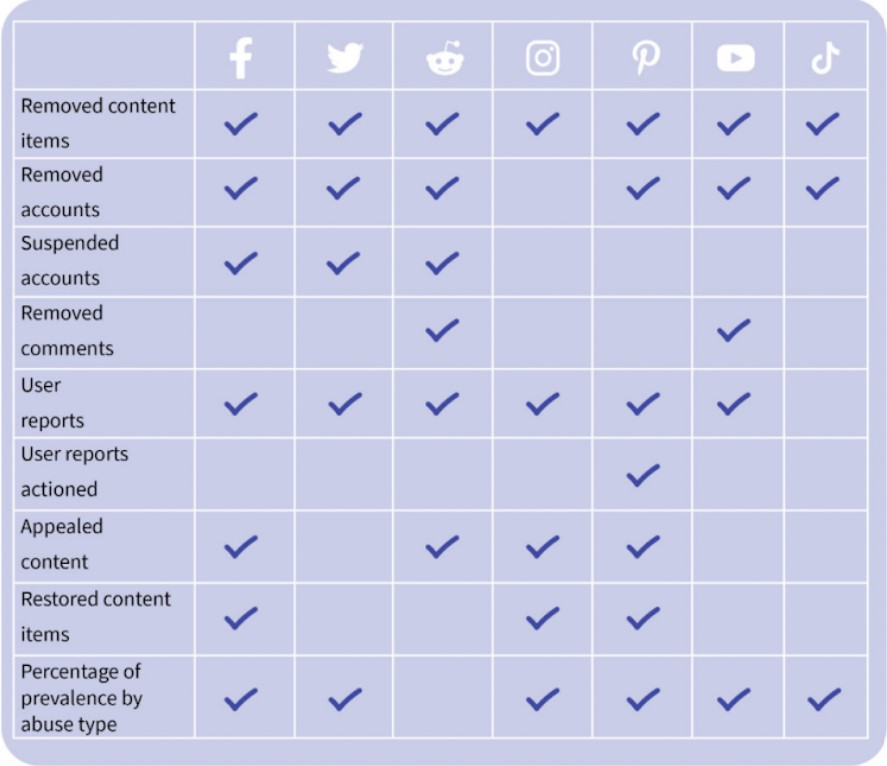
\includegraphics[scale = 0.4]{img/subfig1.jpg}
    \caption{The Guide to Transparency Reports, ActiveFence, 2022. \href{https://www.activefence.com/research/guide-to-transparency-reports/}{https://www.activefence.com/research/guide-to-transparency-reports/}}
\end{figure}

\end{frame}

\begin{frame}{Common Metrics Shared by Social Platforms}
\begin{figure}
    \centering
    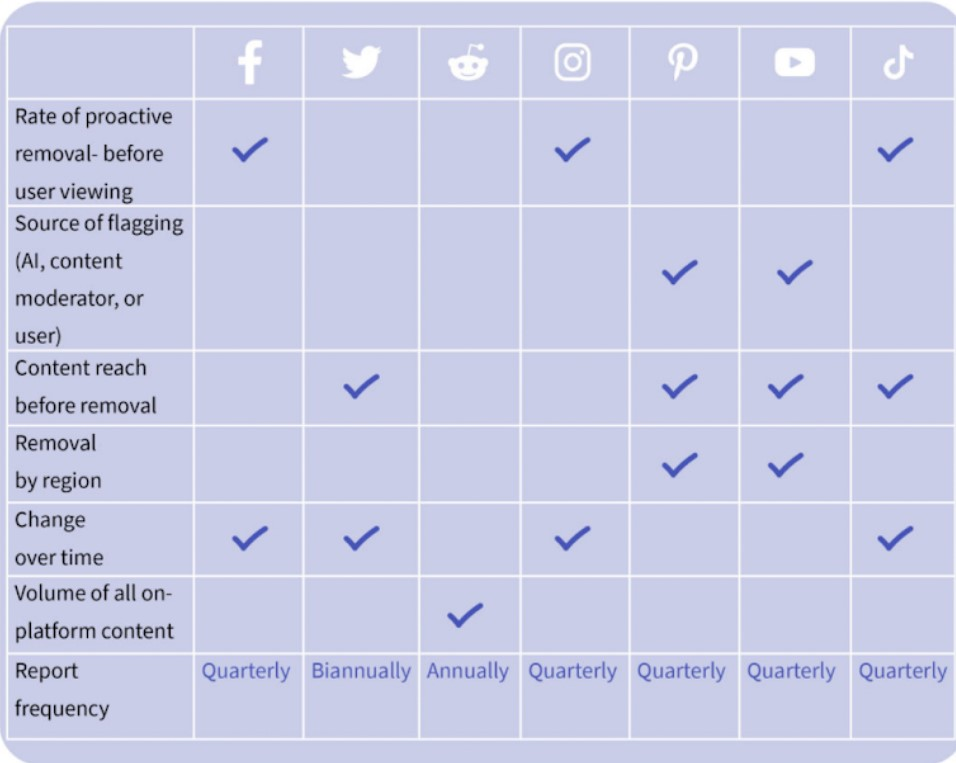
\includegraphics[scale = 0.4]{img/subfig2.jpg}
    \caption{The Guide to Transparency Reports, ActiveFence, 2022. \href{https://www.activefence.com/research/guide-to-transparency-reports/}{https://www.activefence.com/research/guide-to-transparency-reports/}}
\end{figure}

\end{frame}

%%%%%%%%%%%%%%%%%%%%%%%%%%%%%%%%%%%%%%%%%%%%%%%%
%%%%%%%%%%%%%%%%  SLIDE 8  %%%%%%%%%%%%%%%%%%%%%
%%%%%%%%%%%%%%%%%%%%%%%%%%%%%%%%%%%%%%%%%%%%%%%%
\begin{frame}{Other Metrics Examples}
\begin{itemize}
    \item Ecosystem:
    \begin{itemize}
        \item Prevalence: How common are specific types of harmful content?
    
        \begin{itemize}
            \item Number of instances of the category of content posted
            \item Number of users exposed to that category of content
            \item Percentage of content views to that category of content
        \end{itemize}

        \item Severity: How significant and impactful is the harm?

        \begin{itemize}
            \item e.g., “low prevalence, high severity” issues like suicide/self-injury content (versus “high prevalence, low severity” content like clickbait)
        \end{itemize}
    \end{itemize} 
\end{itemize}
\end{frame}

\begin{frame}{Other Metrics Examples}
\begin{itemize}
    \item Operations:

    \begin{itemize}
        \item Enforcement: How quickly are bad content or problematic users removed?

        \begin{itemize}
            \item Time delay between violating content being posted vs. being moderated (\& reach/exposure of that content during “up” period)
        \end{itemize}
    \end{itemize}
    
    \item Quality of decision making (false positives/false negatives)
\end{itemize}
\end{frame}


%%%%%%%%%%%%%%%%%%%%%%%%%%%%%%%%%%%%%%%%%%%%%%%%
%%%%%%%%%%%%%%%%  SLIDE 9  %%%%%%%%%%%%%%%%%%%%%
%%%%%%%%%%%%%%%%%%%%%%%%%%%%%%%%%%%%%%%%%%%%%%%%
\begin{frame}{Developing Metrics}

\begin{itemize}
    \item Metrics are usually developed via two methods:
    \item Behavioral logs

    \begin{itemize}
        \item Based on some definition of an interaction (e.g., users signing up, photos uploaded, comments views, etc.), logs of user behavior are registered in a database
    \end{itemize}

    \item Entity labeling

    \begin{itemize}
        \item Based on some definition of a category (e.g., hate speech, posts about politics, pornographic imagery), content is labeled (usually by human coders, but sometimes via computational systems)
        \item In this second approach, classifiers are then trained on the labeled data, and the output of the classification – when applied more broadly across the system – are registered in a database
    \end{itemize}
\end{itemize}

\end{frame}


%%%%%%%%%%%%%%%%%%%%%%%%%%%%%%%%%%%%%%%%%%%%%%%%
%%%%%%%%%%%%%%%%  SLIDE 10  %%%%%%%%%%%%%%%%%%%%
%%%%%%%%%%%%%%%%%%%%%%%%%%%%%%%%%%%%%%%%%%%%%%%%
\begin{frame}{Metrics Approaches - Behavioral Logs}

\small{
\begin{itemize}
    \item Behavioral log metrics are derived based on a predefined definition (e.g., by one person) and implemented in static code
    \item Example: “views on a post in a feed” could be operationalized as…

    \begin{itemize}
        \item If the post loaded on the device – 0/1 binary
        \item If the post appeared on the device screen – 0/1 binary, based on a threshold cutoff of N milliseconds
        \item How long the post appeared on the device screen – integer/double of N milliseconds
    \end{itemize}
    
    \item We might also consider related metrics:
    
    \begin{itemize}
        \item If the post was recommended to appear in the feed
        \item What position the post was going to appear in the feed
        \item How likely a user is going to interact with the post when it appears
    \end{itemize}
    
    \item Question: Considering all potential measures, how might we operationalize a “good” view of a post?
\end{itemize}
}
\end{frame}


%%%%%%%%%%%%%%%%%%%%%%%%%%%%%%%%%%%%%%%%%%%%%%%%
%%%%%%%%%%%%%%%%  SLIDE 11  %%%%%%%%%%%%%%%%%%%%
%%%%%%%%%%%%%%%%%%%%%%%%%%%%%%%%%%%%%%%%%%%%%%%%
\begin{frame}{Metrics Approaches - Labeling}

\begin{itemize}
    \item Labeling-based metrics, on the other hand, are derived based on a predefined set of criteria (e.g., “guidelines”) where each entity (e.g., content, accounts, etc.) are then categorized according to if they match the criteria
    \item Usually these labels are generated by a group of labelers, and agreement between the labelers determines the final categorization
    \item Then, classifiers (usually machine learning models) are built using the validated, labeled data and projected across a larger dataset. Each entity (content, accounts, etc.) have a likelihood measure of if it matches that category
    \item Sampling methodologies (oversampling abuse)
\end{itemize}
\end{frame}

%%%%%%%%%%%%%%%%%%%%%%%%%%%%%%%%%%%%%%%%%%%%%%%%
%%%%%%%%%%%%%%%%  SLIDE 12  %%%%%%%%%%%%%%%%%%%%
%%%%%%%%%%%%%%%%%%%%%%%%%%%%%%%%%%%%%%%%%%%%%%%%
\begin{frame}{Application of Metrics}
\small{
\begin{itemize}
    \item Metrics based on behavioral logs are relatively straightforward
    \item Metrics based on labeling are much more complicated, because they rely heavily on the sampling of the underlying data, the labels’ validation (quality assurance), and the precision/recall of the classifiers when modeled on the labeled training data… as well as the financial cost of labeling too
    \item Metrics using labeling can be complicated due to:

    
    \begin{itemize}
        \footnotesize{
        \item Choice of sampling methods (and potential issues with oversampling) for choosing what data should be labeled
        \item How well labelers agree (interrater reliability) on if a given entity is labeled correctly – and if this agreement is audited before model training (e.g., creating “golden sets” of training data)
        \item How well a given label can be classified (some classification models perform just better than chance; most classifiers never achieve higher than 80\% accuracy)
        }
    \end{itemize}
\end{itemize}
}
\end{frame}


%%%%%%%%%%%%%%%%%%%%%%%%%%%%%%%%%%%%%%%%%%%%%%%%
%%%%%%%%%%%%%%%%  SLIDE 13  %%%%%%%%%%%%%%%%%%%%
%%%%%%%%%%%%%%%%%%%%%%%%%%%%%%%%%%%%%%%%%%%%%%%%
\begin{frame}{Surveys in T\&S Metrics}

\begin{itemize}
    \item More recently, surveys are increasingly used to develop additional types of measures (\emph{not necessarily metrics}) to look at the attitudes, perceptions, knowledge, or self-reported behaviors of people related to their platform experiences, trust in companies, etc.
    \item Some concepts – e.g., trust – are not possible to measure without surveys, so “tracking surveys” are common ways to understand how things like sentiment might change over time.

    \begin{itemize}
        \item Trust barometer (Edelman) - \href{https://www.edelman.com/trust/2022-trust-barometer}{https://www.edelman.com/trust/2022-trust-barometer}
    \end{itemize}
\end{itemize}
\end{frame}

\begin{frame}{Surveys in T\&S Metrics}

\begin{itemize}
    \item However: surveys are VERY DIFFICULT to use as metrics. They are traditionally hard to move with interventions, difficult to track long-term, and suffer from scalability / representativeness issues. 

    \begin{itemize}
        \item By looking at the associations between surveys and other metrics (both behavioral logs and labeled data), \emph{proxy metrics} can be derived from unique uses of survey data.
    \end{itemize}

    \item {[READING \#4 - International Trust Measurement]}
\end{itemize}
\end{frame}

\begin{frame}{Surveys in T\&S Metrics}

\footnotesize{
\begin{itemize}
    \item More recently, surveys are increasingly used to develop additional types of measures (not necessarily metrics) to look at the attitudes, perceptions, knowledge, or self-reported behaviors of people related to their platform experiences, trust in companies, etc.
    \item Some concepts – e.g., trust – are not possible to measure without surveys, so “tracking surveys” are common ways to understand how things like sentiment might change over time.

    \begin{itemize}
        \footnotesize{
        \item Trust barometer (Edelman) - \href{https://www.edelman.com/trust/2022-trust-barometer}{https://www.edelman.com/trust/2022-trust-barometer}
        }
    \end{itemize}

    \item However: surveys are VERY DIFFICULT to use as metrics. They are traditionally hard to move with interventions, difficult to track long-term, and suffer from scalability / representativeness issues. 

    \begin{itemize}
        \footnotesize{
        \item By looking at the associations between surveys and other metrics (both behavioral logs and labeled data), \emph{proxy metrics} can be derived from unique uses of survey data.
        }
    \end{itemize}

    \item {[READING \#4 - International Trust Measurement]}
\end{itemize}
}
\end{frame}


%%%%%%%%%%%%%%%%%%%%%%%%%%%%%%%%%%%%%%%%%%%%%%%%
%%%%%%%%%%%%%%%%  SLIDE 14  %%%%%%%%%%%%%%%%%%%%
%%%%%%%%%%%%%%%%%%%%%%%%%%%%%%%%%%%%%%%%%%%%%%%%
\begin{frame}{Case studies}

\begin{itemize}
    \item Examples of metrics companies have developed for T\&S work

    \begin{itemize}
        \item Facebook
        \begin{itemize}
            \item MSI
        \end{itemize}
        \item TikTok (\href{https://www.linkedin.com/pulse/graphical-conception-keyword-based-proactivity-ka-tsai-ku/}{source})
    \end{itemize}
    \item {[READING \#3 - Facebook MSI Metric]}
\end{itemize}

\end{frame}


%%%%%%%%%%%%%%%%%%%%%%%%%%%%%%%%%%%%%%%%%%%%%%%%
%%%%%%%%%%%%%%%%  SLIDE 15  %%%%%%%%%%%%%%%%%%%%
%%%%%%%%%%%%%%%%%%%%%%%%%%%%%%%%%%%%%%%%%%%%%%%%
\begin{frame}{Best Practices for Metrics in Practice - Metrics vs. KPI conflict}

\begin{itemize}
    \item Be wary of what a metric tells you, based on how it was operationalized

    \begin{itemize}
        \item \emph{And causation can only be derived from experiments! Don’t assume causality of the associations or potential changes between two metrics.}
    \end{itemize}

    \item Don’t try to optimize for your metrics 
    \item Metrics should inform the goal, not be the goal

    \begin{itemize}
        \item Example: decreasing the number of user reports to 0 isn’t necessarily good, because the number of user reports is not a proxy for how much abuse is on the platform (instead, it is an indicator of ability to submit reports; it might not even be a proxy for how much people understand how to report, confidence in reporting, etc.)
    \end{itemize}
\end{itemize}
\end{frame}

%%%%%%%%%%%%%%%%%%%%%%%%%%%%%%%%%%%%%%%%%%%%%%%%
%%%%%%%%%%%%%%%%  SLIDE 16  %%%%%%%%%%%%%%%%%%%%
%%%%%%%%%%%%%%%%%%%%%%%%%%%%%%%%%%%%%%%%%%%%%%%%
\begin{frame}{Metrics \& Transparency}

\small{
\begin{itemize}
    \item Transparency reports (TRs) are common ways platforms now inform the public about their Trust \& Safety work
    \item But there is actually no industry standard nor government regulation for TRs
    \item Therefore, there are some problems:

    \begin{itemize}
        \footnotesize{
        \item Companies determine what metrics make it into TRs and how to summarize/aggregate numbers
        \item T\&S metrics – and specifically successes – across the industry cannot be compared between platforms (e.g., is Meta doing better than Twitter?), due to lack of shared metrics operationalization
        \item If a given metric in a TR changes over time, it’s not possible to view the progress or improvement of the problem
        \item Metrics in TRs don’t necessity reflect the severity of a given harm

        \begin{itemize}
            \item e.g., misinformation metrics might include both Flat Earth conspiracies, celebrity deaths, and “Stop the Steal” discussions – prior to the January 6th Capitol attack, the 3rd was pretty severe
        \end{itemize}
        }
    \end{itemize}
\end{itemize}
}
\end{frame}


%%%%%%%%%%%%%%%%%%%%%%%%%%%%%%%%%%%%%%%%%%%%%%%%
%%%%%%%%%%%%%%%%  SLIDE 17  %%%%%%%%%%%%%%%%%%%%
%%%%%%%%%%%%%%%%%%%%%%%%%%%%%%%%%%%%%%%%%%%%%%%%
\begin{frame}{Transparency Reports Deep Dive}

\begin{itemize}
    \item What do TRs actually show?

    \begin{itemize}
        \item \textbf{Prevalence:} The percentage of all views of violating content in a particular content category (e.g., hate speech).
        \item \textbf{Proactive Rate:} Out of all content or accounts that the company took action on, the percentage that were flagged by the company’s tools before users flagged them
        \item \textbf{Content/Accounts Actioned}
        \item \textbf{Appealed Content}
        \item \textbf{Restored Content}
    \end{itemize}

    \item {[READING \#5 - Transparency Report Tracking]}
\end{itemize}
\end{frame}

%%%%%%%%%%%%%%%%%%%%%%%%%%%%%%%%%%%%%%%%%%%%%%%%
%%%%%%%%%%%%%%%%  SLIDE 18  %%%%%%%%%%%%%%%%%%%%
%%%%%%%%%%%%%%%%%%%%%%%%%%%%%%%%%%%%%%%%%%%%%%%%
\begin{frame}{Transparency \& Legal Responsibility}

\small{
\begin{itemize}
    \item Beyond the good will of platforms to be transparent, platforms are required to communicate their measures to keep users safe under different online safety regulations
    \item Requirements range from specific to broad, based on regulation e.g.

    \begin{itemize}
        \item EU’s \href{https://digitalservicesact.cc/dsa/art13.html}{DSA} 
        \item \href{https://bills.parliament.uk/publications/49377/documents/2735}{UK’s Online Safety Bill} - broad

        \begin{itemize}
            \item “The information set out in transparency reports is intended to help users understand the steps providers are taking to keep them safe.”
        \end{itemize}

        \item \href{https://www.legislation.gov.au/Details/C2021A00076}{Australia’s online safety act} - “The extent to which the provider complied with the applicable basic online safety expectations during such regular intervals as are specified in the determination.”

        \begin{itemize}
            \item The eSafety commissioner can also issue a transparency notice surrounding a specific theme (\href{https://www.esafety.gov.au/industry/basic-online-safety-expectations/responses-to-transparency-notices\#:~:text=On\%2029\%20August\%202022\%2C\%20eSafety,Meta}{source})
        \end{itemize}
    \end{itemize}
\end{itemize}
}

\note[]{
\begin{itemize}
    \scriptsize{
    \item [] the number of orders received from Member States’ authorities, categorised by the type of illegal content concerned, including orders issued in accordance with Articles 8 (\url {https://digitalservicesact.cc/dsa/art8.html}) and \href{https://digitalservicesact.cc/dsa/art9.html}{9}, and the average time needed for taking the action specified in those orders; 
    
    \item[] the number of notices submitted in accordance with \href{https://digitalservicesact.cc/dsa/art14.html}{Article 14}, categorised by the type of alleged illegal content concerned, any action taken pursuant to the notices by differentiating whether the action was taken on the basis of the law or the terms and conditions of the provider, and the average time needed for taking the action;
    
    \item[] the content moderation engaged in at the providers’ own initiative, including the number and type of measures taken that affect the availability, visibility and accessibility of information provided by the recipients of the service and the recipients’ ability to provide information, categorised by the type of reason and basis for taking those measures;
    
    \item[] the number of complaints received through the internal complaint-handling system referred to in Article 17, the basis for those complaints, decisions taken in respect of those complaints, the average time needed for taking those decisions and the number of instances where those decisions were reversed.
    }
\end{itemize}
}
\end{frame}

%%%%%%%%%%%%%%%%%%%%%%%%%%%%%%%%%%%%%%%%%%%%%%%%
%%%%%%%%%%%%%%%%  SLIDE 19  %%%%%%%%%%%%%%%%%%%%
%%%%%%%%%%%%%%%%%%%%%%%%%%%%%%%%%%%%%%%%%%%%%%%%
\begin{frame}{Transparency Reports in Detail}

\begin{itemize}
    \item Review the following reports, and try to identify what problems might be present when comparing the platforms.

    \begin{itemize}
        \item \href{https://transparencyreport.google.com/youtube-policy/removals?hl=en}{Youtube}
        \item \href{https://transparency.fb.com/data/community-standards-enforcement/}{Facebook}
        \item \href{https://www.tiktok.com/transparency/en/community-guidelines-enforcement-2022-3/}{Tiktok}
    \end{itemize}
\end{itemize}

\textbf{Class Activity}

\begin{itemize}
    \item Transparency Metrics Standardization: What metrics should become an industry standard? How should they be defined and operationalized? Why that way?

    \begin{itemize}
        \item \href{https://www.oecd-vtrf-pilot.org/reports}{Example - OECD}
        \item \href{https://digitalservicesact.cc/dsa/art13.html}{Example  - DSA}
        \item \href{https://docs.google.com/presentation/d/1aWLOVkQQ7YD2dIxrFSF6EF8-t60SwwBj449ytxLITiQ/edit\#slide=id.g16bf9025cd7_0_82}{Example - ActiveFence}
    \end{itemize}
\end{itemize}
\end{frame}


%%%%%%%%%%%%%%%%%%%%%%%%%%%%%%%%%%%%%%%%%%%%%%%%
%%%%%%%%%%%%%%%%  SLIDE 20  %%%%%%%%%%%%%%%%%%%%
%%%%%%%%%%%%%%%%%%%%%%%%%%%%%%%%%%%%%%%%%%%%%%%%
\begin{frame}{Transparency Audits}

\begin{itemize}
    \item Under some regulations, a third-party audit is required (e.g., the \href{https://digitalservicesact.cc/dsa/art28.html}{DSA}).
    \item What do these report audits tell us?

    \begin{itemize}
        \item Example \href{https://about.fb.com/wp-content/uploads/2022/05/EY-CSER-Independent-Assessment-Q4-2021.pdf}{EY audit} on Facebook enforcement of community guidelines. Metrics in scope:

        \begin{itemize}
            \item Prevalence 
            \item Content Actioned 
            \item Proactive Rate 
            \item Appealed Content 
            \item Restored Content 
        \end{itemize}

        \item Are these the right metrics? 
        \item Where are the gaps?

        \begin{itemize}
            \item Hint: UA war, stop the steal (misinformation, propaganda, elections integrity)
        \end{itemize}
    \end{itemize}
\end{itemize}
\end{frame}

%\backpage

\end{document}